\documentclass[12pt]{article}%
\usepackage{amsfonts}
\usepackage{fancyhdr}
\usepackage{comment}
\usepackage[a4paper, top=2.5cm, bottom=2.5cm, left=2.2cm, right=2.2cm]%
{geometry}
\usepackage{times}
\usepackage{amsmath}
\usepackage{changepage}
\usepackage{amssymb}
\usepackage{graphicx}%
\setcounter{MaxMatrixCols}{30}
\newtheorem{theorem}{Theorem}
\newtheorem{acknowledgement}[theorem]{Acknowledgement}
\newtheorem{algorithm}[theorem]{Algorithm}
\newtheorem{axiom}{Axiom}
\newtheorem{case}[theorem]{Case}
\newtheorem{claim}[theorem]{Claim}
\newtheorem{conclusion}[theorem]{Conclusion}
\newtheorem{condition}[theorem]{Condition}
\newtheorem{conjecture}[theorem]{Conjecture}
\newtheorem{corollary}[theorem]{Corollary}
\newtheorem{criterion}[theorem]{Criterion}
\newtheorem{definition}[theorem]{Definition}
\newtheorem{example}[theorem]{Example}
\newtheorem{exercise}[theorem]{Exercise}
\newtheorem{lemma}[theorem]{Lemma}
\newtheorem{notation}[theorem]{Notation}
\newtheorem{problem}[theorem]{Problem}
\newtheorem{proposition}[theorem]{Proposition}
\newtheorem{remark}[theorem]{Remark}
\newtheorem{solution}[theorem]{Solution}
\newtheorem{summary}[theorem]{Summary}
\newenvironment{proof}[1][Proof]{\textbf{#1.} }{\ \rule{0.5em}{0.5em}}

\newcommand{\Q}{\mathbb{Q}}
\newcommand{\R}{\mathbb{R}}
\newcommand{\C}{\mathbb{C}}
\newcommand{\Z}{\mathbb{Z}}

\begin{document}

\title{Fun with Molding}
\author{Solution Key}
\date{\today}
\maketitle
\section{Pattern Transfer (6 points)}

\subsection{Loctite Exposure} Use the Beer-Lambert law to explain why flipping the glass/Loctite/transparency assembly before UV exposure allows for better separation from the transparency and better adhesion to the glass slide.
\newline
\newline
\textbf{Answer:}
\newline
\newline
Beer-Lambert law:
\newline

\begin{equation}
\tau = \sum_{i=1}^{N} \tau_{i} = \sum_{i=1}^{N} \sigma_1 \int_{0}^{l} n_i(z)dz
\end{equation}
\newline

\begin{equation}
A = \sum_{i=1}^{N} A_i = \sum_{i=1}^{N} \epsilon_1 \int_{0}^{l} c_i(z) dz
\end{equation}
\newline
\newline
where $N$ = number of attenuating species in material, $\sigma_i$ = attenuating cross section, $n_i$ = number density, $\epsilon_i$ = molar attenuation coefficient, $c_i$ = amount concentration, $l$ = path length of light beam ($=0.48 \pm 0.01$ mm for this experiment)
\newline
\newline
[1] Beer-Lambert law states that light intensity attenuates when passing through glue: \newline
Longer path length $\rightarrow$ lower transmittance $\rightarrow$ top receives more UV exposure compared to the bottom
\newline
\newline
[1] Loctite is negative photoresist $\rightarrow$ UV strengthens cross-linking $\rightarrow$ Loctite near the glass becomes harder $\rightarrow$ glass-Loctite interface becomes more adhesive than the transparancy-Loctite interface

\subsection{Pattern Resolution} Compare the measured width of the millifluidic channel on the mask and the actual width that was obtained in the Loctite pattern (mean $\pm$ std. dev.). Briefly explain two reasons why the Loctite channel width is different from that of the mask. What two factors impose a lower limit to the pattern resolution? Estimate this size (to an order of magnitude).
\newline
\newline
\textbf{Answer:}
\newline
\newline
[0.5] Mask: 4.05 $\pm$ 0.10 mm
\newline
[0.5] Loctite: 3.22 $\pm$ 0.09 mm
\newline
\newline
Reasons for difference in channel width:
\newline
[0.5] UV light bends around the mask, providing exposure around mask edges
\newline
[0.5] NEED ONE MORE REASON
\newline
\newline
Factors limiting the resolution:
\newline
[0.5] thickness of glue layer
\newline
[0.5] incidence of light from an angle
\newline
\newline
[1] Order of magnitude is around the thickness of the glue layer

\section{Flow Behavior (4 points)}
\subsection{Reynolds Number} What is the (approximate) Reynolds number of the flow in the channel of your device? List/show the values of all parameters and measurements in your calculations. 
\newline
\newline
\textbf{Answer:}
\newline
\begin{equation}
Re = \frac{d \rho \nu}{\mu} = \frac{4A}{p} \frac{\rho v}{\mu}
\end{equation}

\noindent [0.5] Handling error:
\newline
$side1 = x \pm \Delta x$
\newline
$side2 = y \pm \Delta y$
\newline
$A = x * y \pm x*y*(\frac{\Delta x}{x} + \frac{\Delta y}{y})$
\newline
\newline
[0.5] $Re \approx 10-100$ (estimate from video: 5 cm travel in 2 seconds) 
\newline

\subsection{Flow Rate}
Estimate the flow rate required to obtain turbulent flow in the millifluidic device. By how many orders of magnitude is this flow rate higher than the actual flow rate in your experiment?
\newline
\newline
\textbf{Answer:}
\newline
\newline
Turbulent flow at $Re \approx 2300 \rightarrow$ two orders of magnitude higher
\newline
\newline
[0.5] Flow velocity $\approx 3 \frac{m}{s}$
\newline
\newline
[0.5] Flow rate = Flow velocity * area $\approx 4.6 *10^-6 \frac{m^3}{s}$
\newline
\newline
***********************************************************************************
\section{Mixing Behavior (3 points)}

\textbf{Answer:}
Question 3 (3 points)
a)	1 point each for presenting the photographs of lotus, oak, CD. Deduct 0.5 point for omitting scale bar.
\newline
\newline

\section{Design for Mixing (2 points)}

\textbf{Answer:}
Question 4 (4 points). 4 points for reasonable hypotheses. Award 1 point if reasoning is unclear or incorrect.
\newline
\newline


**************************************************************************************
a)	Scouring tends to trap or nucleate bubbles compared to smooth surface so PDMS near scours has bubbles.
b)	Cover prevents air from escaping so air that comes out on heating is trapped in the PDMS.

\subsection{Flow Behavior}
Every word problem has an "unknown number".In this problem,it is the price of the blouse. Always let "x" represent the "unknown number".That is, let "x" answer the question.

\section{Part 2 Write-up}
\subsection {Molding of microstructures}
blah
\newline
\textbf{Answer:}
\newline
\begin{figure} [ht]
\centering
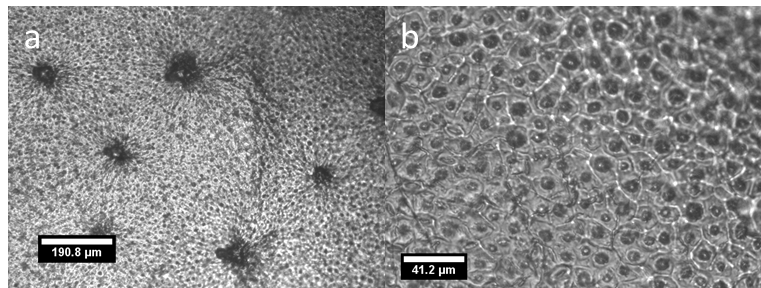
\includegraphics[width=.5\textwidth]{lotus.png}
\caption{\label{fig:lotus}Optical micrographs of PDMS molded on lotus leaf at a) 10x magnification and b) 40x magnification.}
\end{figure}

\begin{figure} [ht]
\centering
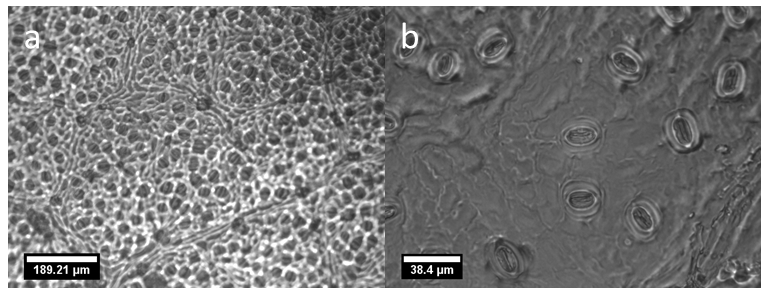
\includegraphics[width=.5\textwidth]{oak.png}
\caption{\label{fig:oak leaf}Optical micrographs of PDMS molded on lotus leaf at a) 10x magnification and b) 40x magnification.}
\end{figure}

\begin{figure} [ht]
\centering
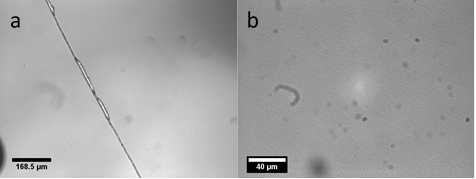
\includegraphics[width=.5\textwidth]{cd.png}
\caption{\label{fig:cd}Optical micrographs of PDMS molded on CD at a) 10x magnification and b) 40x magnification.}
\end{figure}

[3] 1 point each for presenting images of lotus, oak and CD at different magnifications. 0.5 point deducted for omitting scale bar

\subsection {Examining Cured PDMS}
blah
\newline
\textbf{Answer:}
\newline

a) The region of scoring showed trapped bubbles on its features. Scoured regions act as sites for heterogeneous nucleations for air bubbles to form as the PDMS degases.
\newline

[1] Observation of air bubbles at scouring
[1] Heterogeneous nucleation of air bubbles at the site of scouring during degas
\newline

b) The covered sample presented more bubbles in the mixture. Covering the PDMS did not allow for the system to fully degas upon heating.
\newline

[1] Observation of more air bubbles for covered PDMS
[1] Covering PDMS limits the amount of air escaping from PDMS

\end{document}